\chapter{Convolutional Neural Network}

\section{Brief Review of CNN}

CNN is a type of ANN structure designed to handle grid-like data. It is effective when dealing when data spatially correlated, thus becomes very popular in computer vision. It defines ``kernel'' that aggregates nearby pixels information before sending it to a dense network.

A CNN kernel, also known as a filter, is a small matrix of weights that slides across the input image or feature map to perform a mathematical operation called convolution. An demonstration of CNN kernel is given in Fig. \ref{ch:cnn:fig:cnn_kernel}. Multiple kernels can be defined on the same layer to handle the same feature map, each kernel associated with an output channel. In practice, each kernel or channel is designed to detect a specific features in the feature map. For example, there might be a kernel detecting edges, while a second kernel detect color codes.

\begin{figure}
	\centering
	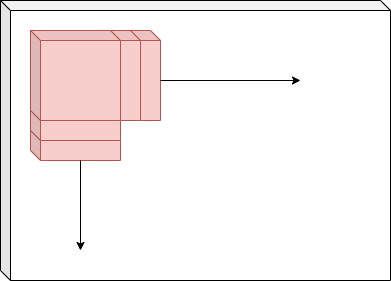
\includegraphics[width=200pt]{chapters/ch-cnn/figs/cnn_general.png}
	\caption{A demonstration of CNN kernel. The input is given by the white box (3D), and the kernel by the red box.} \label{ch:cnn:fig:cnn_kernel}
\end{figure}

Notice that CNN differs quite largely from transformer in the problems they are expected to address. CNN is more for spatial data processing such as image processing, while transformer targets more on sequential data processing such as natural language processing and machine translation.